% !TEX root = ../main.tex

\section{初始节点表示学习}
\label{sec:metartl-pretrain}

设 $\mathcal V_\tau$ 为类型 $\tau\in\mathcal T_v$ 的节点集合，
$D_\tau$ 为对应表格的原始行。MetaRTL 对不同类型分别设置表格神经网络
$f_\tau$，将异构字段编码到共同的 $d$ 维空间。对一个采样批次 $i$，
其类型为 $\tau$ 的节点索引集合记作 $\mathcal B_{\tau}^{(i)}$，初始表示为
\begin{equation}
  X_{\tau}^{(i)}
  = f_\tau\!\left(D_\tau[\mathcal B_{\tau}^{(i)}]\right)
  \in \mathbb R^{|\mathcal B_{\tau}^{(i)}|\times d}.
  \label{eq:metartl-tnn}
\end{equation}
表格编码器处理行内字段，异构图网络处理行间关系，两者承担不同的建模职责。
该设计与基于表格编码器和异构 GraphSAGE 的关系深度学习基线具有可比性
\cite{fey2024rdl,hamilton2017graphsage}。

第一阶段从训练种子出发采样小批次子图
$\mathcal G_i=(\mathcal V_i,\mathcal E_i)$，并用两层异构图网络聚合不同关系
类型的邻域信息。若 $g_{\omega}$ 表示异构图网络，$q_{\psi}$ 为任务预测头，
则预训练目标可写为
\begin{equation}
  \min_{\theta,\omega,\psi}
  \sum_{i\in\mathcal I_{\mathrm{train}}}
  \mathcal L_{\mathrm{task}}\!\left(
    q_\psi\!\left(g_\omega(
      \{f_{\tau,\theta}(D_\tau[\mathcal B_\tau^{(i)}])\}_{\tau},
      \mathcal G_i)\right),\,Y_i
  \right),
  \label{eq:metartl-pretrain}
\end{equation}
其中 $\mathcal L_{\mathrm{task}}$ 表示与预测任务对应的损失函数。
实验中预训练阶段进行五个训练轮次，其目的在于得到可供路径传播的节点
初始表示，而非将浅层图网络的输出直接作为最终结果。
预训练结束后，使用训练得到的表格编码器为后续阶段涉及的节点生成
$X_\tau\in\mathbb R^{|\mathcal V_\tau|\times d}$，并在第二阶段固定这些初始表示。

\section{基于元路径的非参数特征传播}
\label{sec:metartl-metapath}

元路径是定义在关系模式上的类型序列
\begin{equation}
  \mathcal P:\quad
  \tau_s=\tau_0\longrightarrow\tau_1\longrightarrow\cdots
  \longrightarrow\tau_\ell=\tau_t,
  \label{eq:metartl-path}
\end{equation}
其中 $\tau_s$ 和 $\tau_t$ 分别为源类型和预测目标类型。不同的类型序列
对应不同的跨表语义，例如“论文—作者—机构”与“论文—作者—论文”
即使有共同的起点，也描述不同的关联\cite{dong2017metapath2vec}。
令 $A_{\tau_j\leftarrow\tau_{j-1}}$ 为沿相应关系从
$\tau_{j-1}$ 聚合到 $\tau_j$ 的度归一化矩阵，则路径 $\mathcal P$ 的
传播矩阵为
\begin{equation}
  A^{\mathcal P}
  =A_{\tau_t\leftarrow\tau_{\ell-1}}\cdots
   A_{\tau_2\leftarrow\tau_1}
   A_{\tau_1\leftarrow\tau_s}.
  \label{eq:metartl-path-adj}
\end{equation}
这一乘积描述沿指定关系序列的特征传递，不含需要反向传播更新的参数。
在数据准备阶段复用较短路径的中间结果，得到候选元路径的传播矩阵，
再在训练批次中按目标节点和可用源节点索引截取。设
$\mathcal B_t$ 为批次目标节点，$\mathcal B_s$ 为该路径涉及的源节点，
则对应的批次特征为
\begin{equation}
  H_{\mathcal P}^{(\mathcal B)}
  =A^{\mathcal P}[\mathcal B_t,\mathcal B_s]\,
   X_{\tau_s}[\mathcal B_s,:]
  \in\mathbb R^{|\mathcal B_t|\times d}.
  \label{eq:metartl-path-feature}
\end{equation}
若 $\mathcal B_s$ 未覆盖路径矩阵中所有非零源节点，该式表示相应批次范围内的
路径特征；批次采样范围因此也是实验配置的一部分。将零跳路径定义为
$H_0=X_{\tau_t}[\mathcal B_t,:]$，可同时保留目标表自身字段信息。

与在每轮训练中反复执行深层可训练邻域传播相比，路径矩阵可跨训练轮次复用。
不过，矩阵乘积可能产生比原始边集更稠密的中间结果，因此这种预计算并非
无条件地节省时间或内存；其实际成本取决于关系模式、最大跳数、非零元数量
和存储策略。

\section{MetaAttn 路径语义融合}
\label{sec:metartl-attn}

MetaAttn 由元路径自注意力和全局节点交叉注意力两条分支组成，如
图~\ref{fig:metartl-metaattn} 所示。前者选择不同连接路径承载的信息，
后者使批次中的目标节点访问跨批共享的原型表示。

\begin{figure}[htbp]
  \centering
  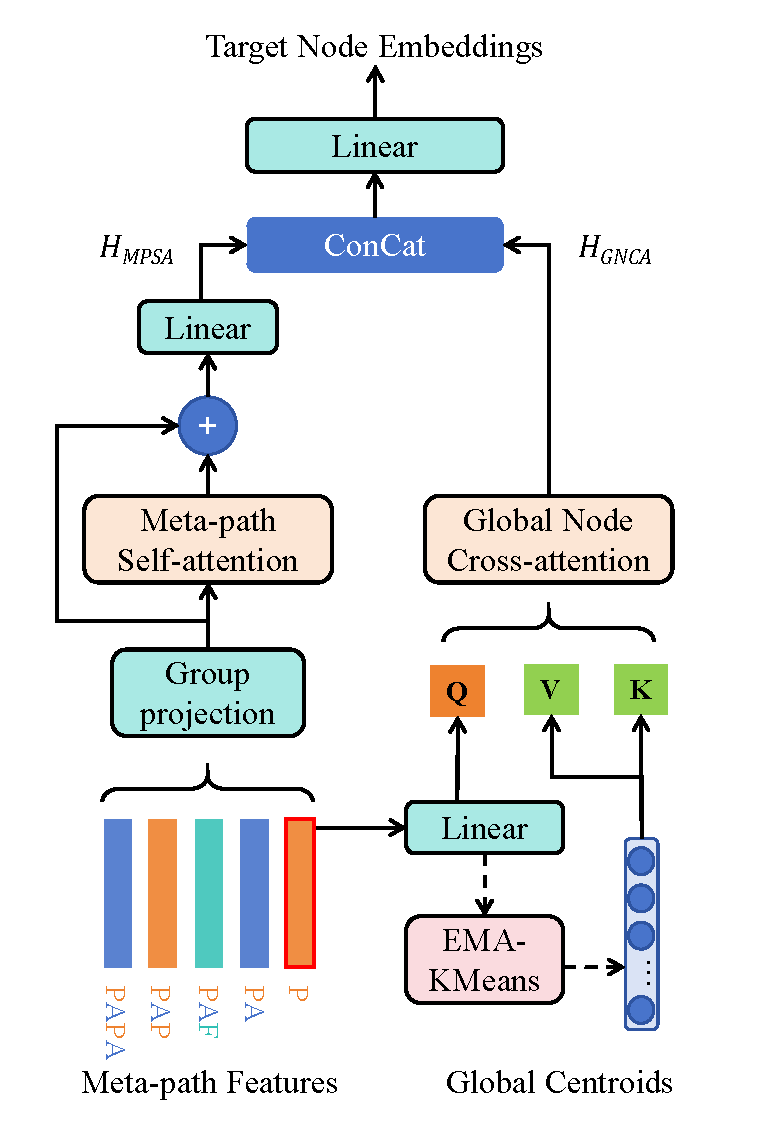
\includegraphics[width=0.50\textwidth]{figures/metartl/fig22.pdf}
  \caption{MetaAttn 的路径自注意力与共享原型交叉注意力结构}
  \label{fig:metartl-metaattn}
\end{figure}

\subsection{元路径自注意力}

令 $\Phi$ 为候选元路径集合，$m=|\Phi|$。对每一条路径的特征
$H_{\mathcal P}^{(\mathcal B)}$，按照其源节点类型 $\tau_s(\mathcal P)$
应用类型特定线性映射，并沿路径维堆叠，得到
\begin{equation}
  Z_{\mathcal B}
  =\operatorname{Stack}_{\mathcal P\in\Phi}
  \!\left(
    H_{\mathcal P}^{(\mathcal B)}
    W_{\tau_s(\mathcal P)}+b_{\tau_s(\mathcal P)}
  \right)
  \in\mathbb R^{|\mathcal B_t|\times m\times d}.
  \label{eq:metartl-stack}
\end{equation}
这样，同一源表类型可共享线性映射，而每条路径仍保留独立的位置。
对于每个目标节点，以其 $m$ 条路径特征为注意力序列，执行
\begin{equation}
  \operatorname{Attn}(Q,K,V)
  =\operatorname{softmax}\!\left(\frac{QK^\top}{\sqrt d}\right)V.
  \label{eq:metartl-attn}
\end{equation}
自注意力为不同路径建立依赖关系\cite{vaswani2017attention}。
将结果与输入作残差相加，再经过路径维聚合及线性投影，得到
\begin{equation}
  H_{\mathrm{MPSA}}
  =\operatorname{Proj}_{\Phi\rightarrow d}
  \!\left(\operatorname{SelfAttn}(Z_{\mathcal B})+Z_{\mathcal B}\right)
  \in\mathbb R^{|\mathcal B_t|\times d}.
  \label{eq:metartl-mpsa}
\end{equation}
其中 $\operatorname{Proj}_{\Phi\rightarrow d}$ 为作用于路径维的
可训练投影，将每个目标节点的多条路径表示映射为一个 $d$ 维向量。

\subsection{全局节点交叉注意力与输出}

仅从采样批次取得路径特征可能遗漏批次外的语义。MetaAttn 因此维护
$c$ 个跨批共享的原型向量
$C\in\mathbb R^{c\times d}$，以零跳目标节点特征作为查询，
以原型作为键和值，计算
\begin{equation}
  H_{\mathrm{GNCA}}
  =\operatorname{CrossAttn}(H_0W_Q,\;C,\;C).
  \label{eq:metartl-gnca}
\end{equation}
训练过程中采用基于 K-Means 的指数滑动平均规则，根据目标节点特征
更新 $C$。原型在批次之间共享，使目标节点能够利用批次外的统计信息，
同时避免与全图所有节点逐一计算注意力。
这一分支与使用共享全局节点的图注意力设计有关\cite{kong2023goat}。

两条分支的输出拼接后，由线性层生成最终目标节点表示：
\begin{equation}
  H_{\mathrm{out}}
  =W_F[H_{\mathrm{MPSA}}\Vert H_{\mathrm{GNCA}}]+b_F,
  \qquad
  \widehat Y=q(H_{\mathrm{out}}).
  \label{eq:metartl-output}
\end{equation}
第二阶段固定初始节点表示，并通过任务损失函数优化类型映射、
注意力模块与预测头的参数。预测头根据分类或回归任务设置，
分别输出类别预测值或连续数值。

\section{计算特征与方法边界}
\label{sec:metartl-complexity}

从消息传递的角度，可以把式~\eqref{eq:metartl-path-adj} 展开为
\begin{equation}
  H_{\mathcal P}^{(0)}=X_{\tau_s},\qquad
  H_{\mathcal P}^{(j)}
  =A_{\tau_j\leftarrow\tau_{j-1}}H_{\mathcal P}^{(j-1)},
  \quad j=1,\ldots,\ell.
  \label{eq:metartl-recursion}
\end{equation}
由矩阵乘法的结合律，
$H_{\mathcal P}^{(\ell)}=A^{\mathcal P}X_{\tau_s}$。
因此，长度为 $\ell$ 的元路径传播可解释为 $\ell$ 步沿指定关系类型
的无参数消息聚合，MetaAttn 则对多个路径的结果进行可训练融合。
全局节点交叉注意力使用共享原型而非数据库边，属于补充的
跨批信息通道，不能简单等同于同一图上的邻接消息传递。

设一个训练轮次中处理的目标节点总数为 $n_t$，路径数为 $m$，原型数为 $c$。
在隐藏维度为 $d$ 且常规稠密注意力实现下，路径自注意力及类型映射的
计算量约为
$\mathcal O\!\left(n_t(m^2d+md^2)\right)$；
目标节点到 $c$ 个原型的注意力另需约
$\mathcal O(n_tcd)$ 的相似度与加权计算。
预训练阶段的代价由表格编码器的字段处理以及采样边上的两层消息传递构成，
不能只用图边数表征。

离线路径矩阵的计算量和内存量还取决于
$\sum_{\mathcal P\in\Phi}\operatorname{nnz}(A^{\mathcal P})$
及中间稀疏矩阵乘积的非零元增长。因而，只有在路径集合和关系稀疏度
得到控制时，才能期待该阶段保持较好的可扩展性。本章后面的时间曲线
检验了固定平均出度的合成图设置；它不等同于所有关系数据库上的
复杂度保证。
